\section{Examples}

\subsection{Examples of fo tree-to-tree transductions}\label{sec:appendix-example-fo-transductions}
\begin{example}\label{ex:pre-order}
    Consider a ranked alphabet
    \mypic{21}
    and the tree-to-tree function which does a pre-order traversal of the input tree, as described in the following picture:
    \mypic{30}
     The above function is first-order tree-to-tree transduction. We use four copies of the input tree: one for the binary gray nodes, two for the gray nodes of arity zero, and one for the nodes of the input tree. The key observation is that the pre-order  is first-order definable: a node $x$ is before $y$ in the pre-order if either $x \le y$, or there exist nodes $x',y'$ such that 
     \begin{align*}
         x' \le x \quad \land \quad  y' \le y \quad \land \quad \underbrace{\forall z \ z < x' \Leftrightarrow z < y'}_{\text{$x',y'$ are siblings}} \quad \land \quad \underbrace{\bigvee_{i<j}\child i (x') \land \child j(y').}_{\text{$x'$ is an earlier sibling than $y'$}}
     \end{align*}
     Note that the disjunction over  $i<j$ is finite, since the maximal arity of nodes is determined by the alphabet. 
\end{example}

\subsection{Examples of derivable functions}\label{sec:AppendixExamples}
To illustrate derivable functions, we present a series of examples, some of them will be useful later.


\noindent \begin{example}[Tree homomorphisms]\label{ex:morphism} 
Given two types $\rSigma, \rGamma$ and an arity preserving  function $\ranked{f:\Sigma\to\tmonad\Gamma}$, we can lift $\ranked{f}$ to the tree homomophism  $\ranked{\mathsf{Hom}_f:\tmonad\Sigma\to \tmonad\Gamma}$ which replaces every node by the term corresponding to its label. If $\ranked{f}$ is derivable, then so is  $\ranked{\mathsf{Hom}_f}$. To see this, we use the composition of the two basic functions
\begin{align*}
\ranked{\tmonad\Sigma\xrightarrow{\tmonad f}\tmonad\tmonad\Gamma \xrightarrow{\flatt_\Gamma} \tmonad \Gamma}
\end{align*}
\end{example}

\noindent\begin{example}[Filter]\label{ex:filter} Consider the types $\rGamma, \rSigma$  where $\rGamma$ is a finite type of unary symbols. Consider the function:
$$ \ranked{f:\tmonad (\rSigma+\rGamma)\to\tmonad \rSigma}$$
which erases the elements of $\rGamma$ from the input term. This function is well defined since erasing unary symbols does not break the tree structure of the input.
Let us explain why this is a derivable function.
Consider the basic functions $\ranked{\unit_\rSigma:\rSigma\to\tmonad\rSigma}$ and the constant function $\ranked{\mathsf{empty}:\rGamma\to\tmonad\rSigma}$ which associates to every element of $\rGamma$ the empty term. We compose the following two functions 
\begin{align*}
\xymatrix{
    \ranked{\rSigma+\rGamma}\quad \ar[r]^-{\ranked{\unit_\Sigma+\mathsf{empty}}} & \quad \ranked{\tmonad\rSigma+\tmonad\rSigma}\ar[r]^-{\ranked{\mathrm{forget}}} &\tmonad\rSigma
},
\end{align*}
Then we lift the obtained function to terms, and compose the result with the $\flatt$ function to obtain our function $\ranked{f}$.  
\end{example}

\noindent \begin{example}[Parent and children]\label{ex:sibling}  Let $\rGamma$ be a finite type. We define $\ranked{\rGamma_0}$  to be the ranked set obtained from $\rGamma$ by setting the arity of every element to $0$.  
\medskip
Consider the function:
$$\ranked{ \mathsf{Parent}: \tmonad \rGamma \to \tmonad (\rGamma\otimes (\rGamma_0+0))}$$
which adds to every node of a term in $\tmonad \rSigma$ the label  of its parent if it has one, and $0$ if it is the root.

% from  $(\rGamma\cup\bot)^{\leq n}$, whose lenght is the arity of the node, and such that the $i^{th}$ element of the  list is the symbol of its $i^{th}$ sibling if it has one, otherwise it is $\bot$.
Let us explain how $\ranked{\mathsf{Parent}}$ can be derived. To illustrate this construction, we use the following term over the alphabet $\ranked{\set{1+2+3}}$ as a running example.
\begin{center}
		 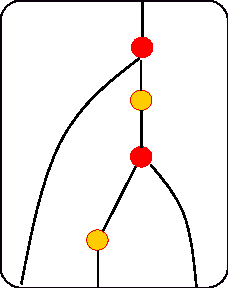
\includegraphics[scale=.6]{parent-1.pdf}
		\end{center}
We denote by $\ranked{\Gamma_1}$ the ranked set obtained from $\rGamma$ by setting the arity of every element to $1$. If $a$ is a element of $\rGamma$, we denote by $a_1$ the corresponding element of $\ranked{\Gamma_1}$. In our example, the alphabet $\ranked{\Gamma_1}$ is
\begin{center}
		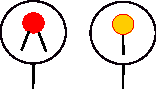
\includegraphics[scale=.5]{parent-2.pdf}
		\end{center}
\begin{enumerate}
\item  First, we apply the homomorphism 
\begin{align*}
\ranked{\mathsf{Hom}_g:\tmonad\Gamma\to \tmonad(\Gamma+\Gamma_1+1)}
\end{align*}
where $\ranked{g}$ is defined on the elements of $\rGamma$ as follows
\begin{align*}
\ranked{g: \Gamma} & \ranked{\to  \tmonad(\Gamma+\Gamma_1+1 )}\\
      a & \mapsto a\tensorpair{1\tensorpair{a_1\tensorpair{0}},\dots, 1\tensorpair{a_1\tensorpair{0}}}
\end{align*}
In our example, the action of $\ranked{g}$ on the elements of $\rGamma$ looks like this
\begin{center}
		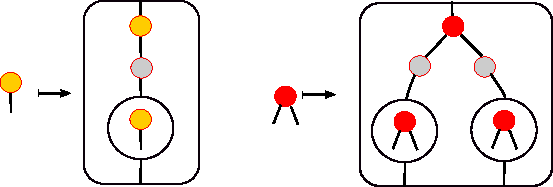
\includegraphics[scale=.5]{parent-3.pdf}
				\end{center}
Hence, after the application of the homomorphism $\ranked{\mathsf{Hom}_g}$, our initial term becomes
\begin{center}
		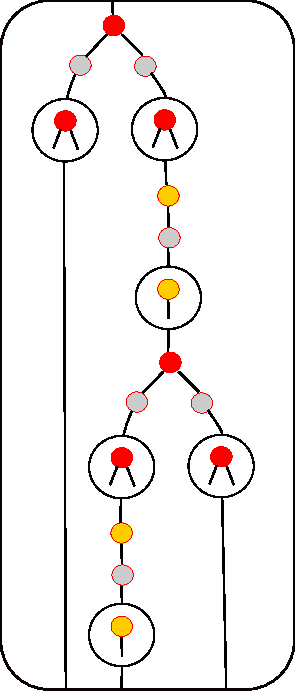
\includegraphics[scale=.5]{parent-4.pdf}
		\end{center}
\item We apply the factorization 
\begin{align*}
\ranked{\ancfact: \tmonad(\Gamma+\Gamma_1+1) \to \tmonad(\tmonad(\Gamma+\Gamma_1)+\tmonad 1)}
\end{align*}
 to separate the symbol $1$ form the other symbols. After this operation, each node lies in the same factor as (the element of $\ranked{\Gamma_1}$ representing) its parent. In our example, the obtained term is the following
\begin{center}
		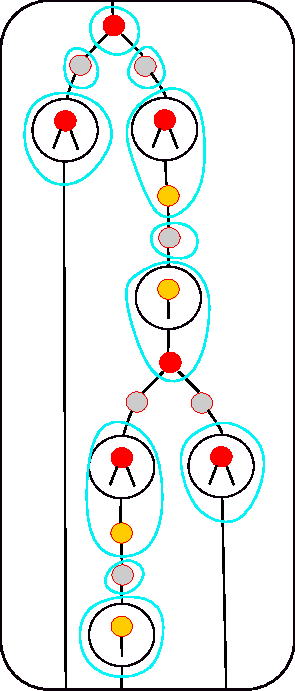
\includegraphics[scale=.5]{parent-5.pdf}
		\end{center}
\item Consider the function 
\begin{align*}
\ranked{h: \tmonad 1 \to \tmonad((\Gamma+\Gamma_1)\otimes(\Gamma_0+0))}
\end{align*}
which is the empty term constant function. It is derivable by lifting the empty term constant function over $1$ to terms.
And let $k$ be the function
\begin{align*}
\ranked{k: \tmonad(\Gamma+\Gamma_1) \to \tmonad((\Gamma+\Gamma_1)\otimes(\Gamma_0+0))}
\end{align*}
which is the identity function, except for the following terms in which it is defined as follows
$$\begin{array}{rll}
a\tensorpair{0,\dots, 0}& \mapsto & \tensorpair{a,0}\tensorpair{0,\dots,0}\\
b_1\tensorpair{a\tensorpair{0,\dots,0}}&\mapsto& \tensorpair{a,b_0}\tensorpair{0,\dots,0}\\
b_1\tensorpair{0} &\mapsto& 0
\end{array}$$
\end{enumerate}
We apply the function $\ranked{h}$ to the factors $\ranked{\tmonad 1}$ and the function $\ranked{k}$ to the factors $\ranked{\tmonad(\rGamma+\rGamma_1)}$. Doing so, we obtain a term in $\ranked{\tmonad\tmonad((\Gamma+\Gamma_1)\otimes(\Gamma_0+0))}$, which we flatten, then we erase the symbols $\ranked{\Gamma_1}$ using the function $\mathsf{Filter}$ of Example~\ref{ex:filter} to obtain the desired term. 
	

\smallskip
If $\rGamma$ is a finite ranked set, we define $\ranked{\Gamma^*}$ as
$$\coprod_{i \leq \text{ maximal arity in } \rGamma} \underbrace{\ranked{\rGamma\otimes \cdots \otimes \rGamma}}_{i\text{ times}}$$
Now consider the function $$\ranked{\mathsf{Children}:\tmonad\rGamma\to \tmonad (\rGamma\otimes (\rGamma_0+0)^*)}$$ which tags every node of a term in $\tmonad \rGamma$ by the list  of its children symbols. When a child is a port, it is marked by $0$ in the list.
The function $\ranked{\mathsf{Children}}$ can be derived using a similar construction as above.
\end{example}



\noindent  \begin{example}[Root and leaves] Let $\rSigma$ be a finite type and $\ranked{f:\rSigma \to \rGamma}$, $\ranked{g: \rSigma \to \rGamma}$ be derivable functions. The function $$\ranked{\mathsf{Root}_{f,g} : \tmonad\rSigma \to \tmonad\rGamma}$$
which applies $\ranked{f}$ to the root and $\ranked{g}$ to the rest of the tree is a derivable function.
To show this, we first start by applying the function $\ranked{\mathsf{Parent}}$. Doing so, the root can be distinguished from the other nodes since it will be tagged by $0$.  

The function $\ranked{h}$ defined below is derivable since its domain is finite. 
\begin{align*}
\ranked{h:\rSigma\otimes(\rSigma_0+0)}&\ranked{\to \rGamma}\\
  \tensorpair{a,0} &\mapsto f(a) \\
  \tensorpair{a,b} &\mapsto g(a) \text{ if } b\neq 0.
\end{align*}
We lift $\ranked{h}$ to terms to conclude.

\smallskip
Similarly, the function $$\ranked{\mathsf{Leaves}_{f,g} : \tmonad\rSigma \to \tmonad\rGamma}$$
 which applies $\ranked{f}$ to the leaves and $\ranked{g}$ to the rest of the tree is derivable. This is done using the same ideas as before, but invoking the function $\ranked{\mathsf{Children}}$ instead of the function $\ranked{\mathsf{Parent}}$: leaves can be distinguished from the other nodes since they are tagged either by a list of $0$ or the empty list.
\end{example}


\noindent\begin{example}[Descendants and ancestors]\label{ex:descendant} If $\rSigma$ is a finite type and $\rGamma\subseteq \rSigma$, then the functions 
\begin{itemize}
\item $\ranked{\mathsf{Descendant}_\rGamma: \tmonad \rSigma \to \tmonad (\rSigma+\rSigma)}$ which replaces the label of each node by its first or second copy, depending on whether it has a descendant in $\rGamma$,
\item $\ranked{\mathsf{Ancestor}_\rGamma: \tmonad \rSigma \to \tmonad (\rSigma+\rSigma)}$ which replaces the label of each node by its first or second copy, depending on whether it has a descendant in $\rGamma$,
\end{itemize}
are derivable.

To derive $\ranked{\mathsf{Descendant}_\rGamma}$, we start by applying the factorization $$\ranked{\decfact: \tmonad\rSigma\to \tmonad(\tmonad\rGamma+\tmonad(\rSigma\setminus\rGamma))}$$ which regroups the elements of $\rSigma$ and the elements of $\ranked{\rSigma\setminus\rGamma}$ into factors depending on whether they have the same ancestors of the same type.

% as in the following figure, where $\rGamma$ is represented by the blue nodes and $\ranked{\rSigma\setminus \rGamma}$ by the yellow ones:
%\begin{center}
%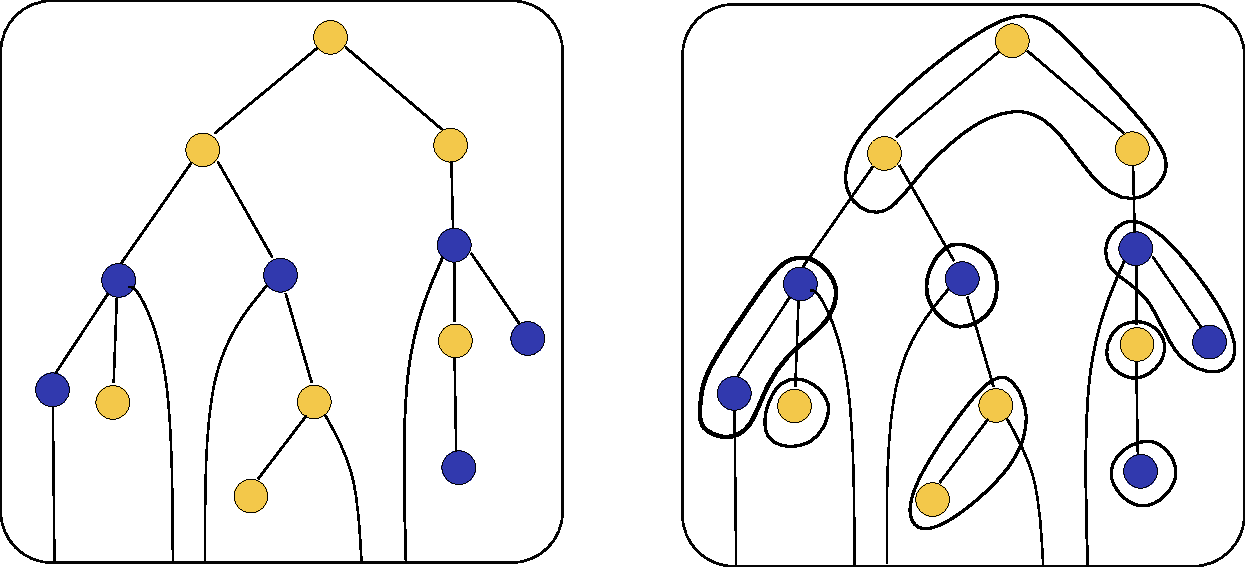
\includegraphics[scale=.3]{descendant.pdf}
%\end{center}
Obviously, all the nodes of the $\rGamma$ factors have a descendant in $\rGamma$. 
In the $\ranked{\rSigma\setminus\rGamma}$ factors which are not leaves in the factorized term, all the nodes have a $\rGamma$ descendant in the original term. To show this, take $f$ to be one of these factors, and suppose by contradiction that one of its nodes does not have a descendant in $\rGamma$. By definition of $\ancfact$, all the elements of $f$ do not have a descendant in $\rGamma$ as well. Since $f$ is not a leaf, it has a child $g$. The factor $g$ cannot be a $\rGamma$
factor as the nodes of $f$ would have a descendant in $\rGamma$. The factor $g$ is then necessarily  a $\ranked{\rSigma\setminus \rGamma}$ factor. If a node of $g$ has a descendant in $\rGamma$, this would give a $\rGamma$ descendant to one of the node of $f$. Thus all the nodes of $g$ are in $\ranked{\rSigma\setminus \rGamma}$ and do not have a descendant in $\rGamma$, meaning that $f$ and $g$ are actually the same factor, which gives a contradiction. Finally, the $\ranked{\rSigma\setminus\rGamma}$ factors which are leaves do not have a descendant in $\rGamma$. With these observations, we can now implement $\mathsf{Descendant}_\rGamma$. 

Let us consider the functions 
$$\begin{array}{llll}
\ranked{\mathsf{Yes}_\rGamma :} & \rGamma &\ranked{\to} &\ranked{ \rSigma+\rSigma}\\
 \ranked{\mathsf{Yes}_{\ranked{\rSigma\setminus\rGamma}:}}& \ranked{\rSigma\setminus\rGamma}&\ranked{\to} &\ranked{ \rSigma+\rSigma}\\
\ranked{\mathsf{No}_{\ranked{\rSigma\setminus\rGamma}: }}&\ranked{\rSigma\setminus\rGamma} &\ranked{\to}& \ranked{ \rSigma+\rSigma}
\end{array}$$
which replaces the label of each node by its first copy for $\ranked{\mathsf{Yes}_\Gamma}$ and $\ranked{\mathsf{Yes}_{\rSigma\setminus\rGamma}}$, and by its second copy for $\ranked{\mathsf{No}_{\rSigma\setminus\rGamma}}$. The three functions are derivable as their domains are finite. 
Consider the functions 
\begin{align*}
\ranked{f:=} &\ranked{ \tmonad\mathsf{Yes}_\rGamma +\tmonad\mathsf{No}_{\rSigma\setminus \rGamma}}\ranked{: \tmonad\rGamma+\tmonad(\rSigma\setminus\rGamma) \to \tmonad (\rSigma+\rSigma)}
\\
\ranked{g:=} & \ranked{ \tmonad\mathsf{Yes}_\rGamma
+\tmonad\mathsf{Yes}_{\rSigma\setminus \rGamma}}\ranked{: \tmonad\rGamma+\tmonad(\rSigma\setminus\rGamma) \to \tmonad (\rSigma+\rSigma)} 
\end{align*}
The descendant function is obtained by applying $\ranked{\mathsf{leaves}_{f,g}}$ followed by a flattening.

\smallskip
To derive the function $\ranked{\mathsf{Ancestor}_\Gamma}$, we apply first a the factorization
\begin{align*}
\ranked{\ancfact: \tmonad\rSigma\to \tmonad(\tmonad\rGamma+\tmonad(\rSigma\setminus\rGamma))}
\end{align*} which regroups the elements of $\rSigma$ and the elements of $\ranked{\rSigma\setminus\rGamma}$ into factors depending on whether they have the same descendants of the same type. 
Using similar arguments as before, we can conclude that:
\begin{itemize}
\item The nodes inside $\rGamma$ factors have $\rGamma$ ancestors.  
\item If a $\ranked{\rSigma\setminus\rGamma}$ factor is the root of the factorized term, then its nodes do not have a $\rGamma$ ancestor.
\item   If a $\ranked{\rSigma\setminus\rGamma}$ factor is not the root of the factorized term, then its nodes do have a $\rGamma$ ancestor.
\end{itemize}
The ancestor function is obtained by applying $\ranked{\mathsf{root}_{f,g}}$ followed by a flattening.
\end{example}

\noindent\begin{example}[Partial unfold]\label{ex:partial-shallow-unfold} If $\rGamma$ and $\rDelta$ are types, we define $\ranked{\Gamma*\Delta}$ to be $\ranked{\Gamma.(1+\Delta)}$. We call its inhabitants the \emph{partial shallow} terms. A partial shallow term looks like this, where we omitted to draw the element 1:
\begin{center}
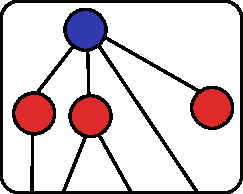
\includegraphics[scale=.4]{partial-shallow-term.pdf}
\end{center}
We define the partial shallow unfolding functions to be the function of type
\begin{align*}
\ranked{{\reduce k \Sigma}*{\Gamma^k} \to \reduce k ({\Sigma}*{\Gamma})} 
\end{align*}
 \begin{center}
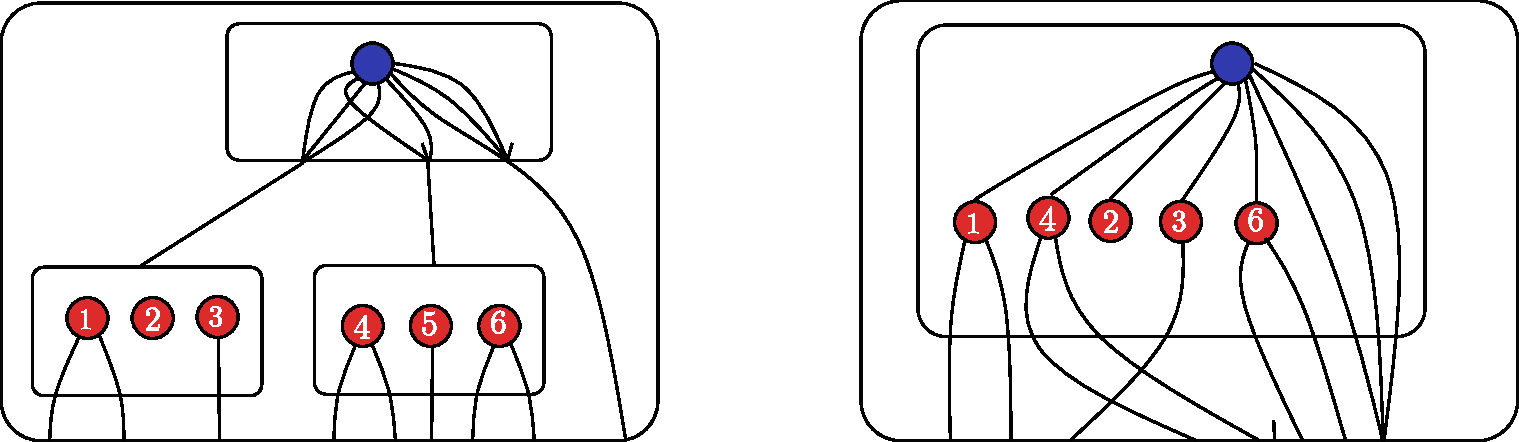
\includegraphics[scale=.4]{partial-shallow-unfold.pdf}
 \end{center}
\end{example}

\noindent\begin{example} Consider the function $\ranked{f}$ 
 \begin{align*}
\ranked{f : \tmonad \Sigma^{[k]} \rightarrow  (\tmonad \Sigma)^{[k]}}
\end{align*}
which coincides with the unfolding function when restricted to a very specific class of inputs: the image of every twist is a singleton. Below is an example illustrating the function $\ranked{f}$ 
  \begin{center}
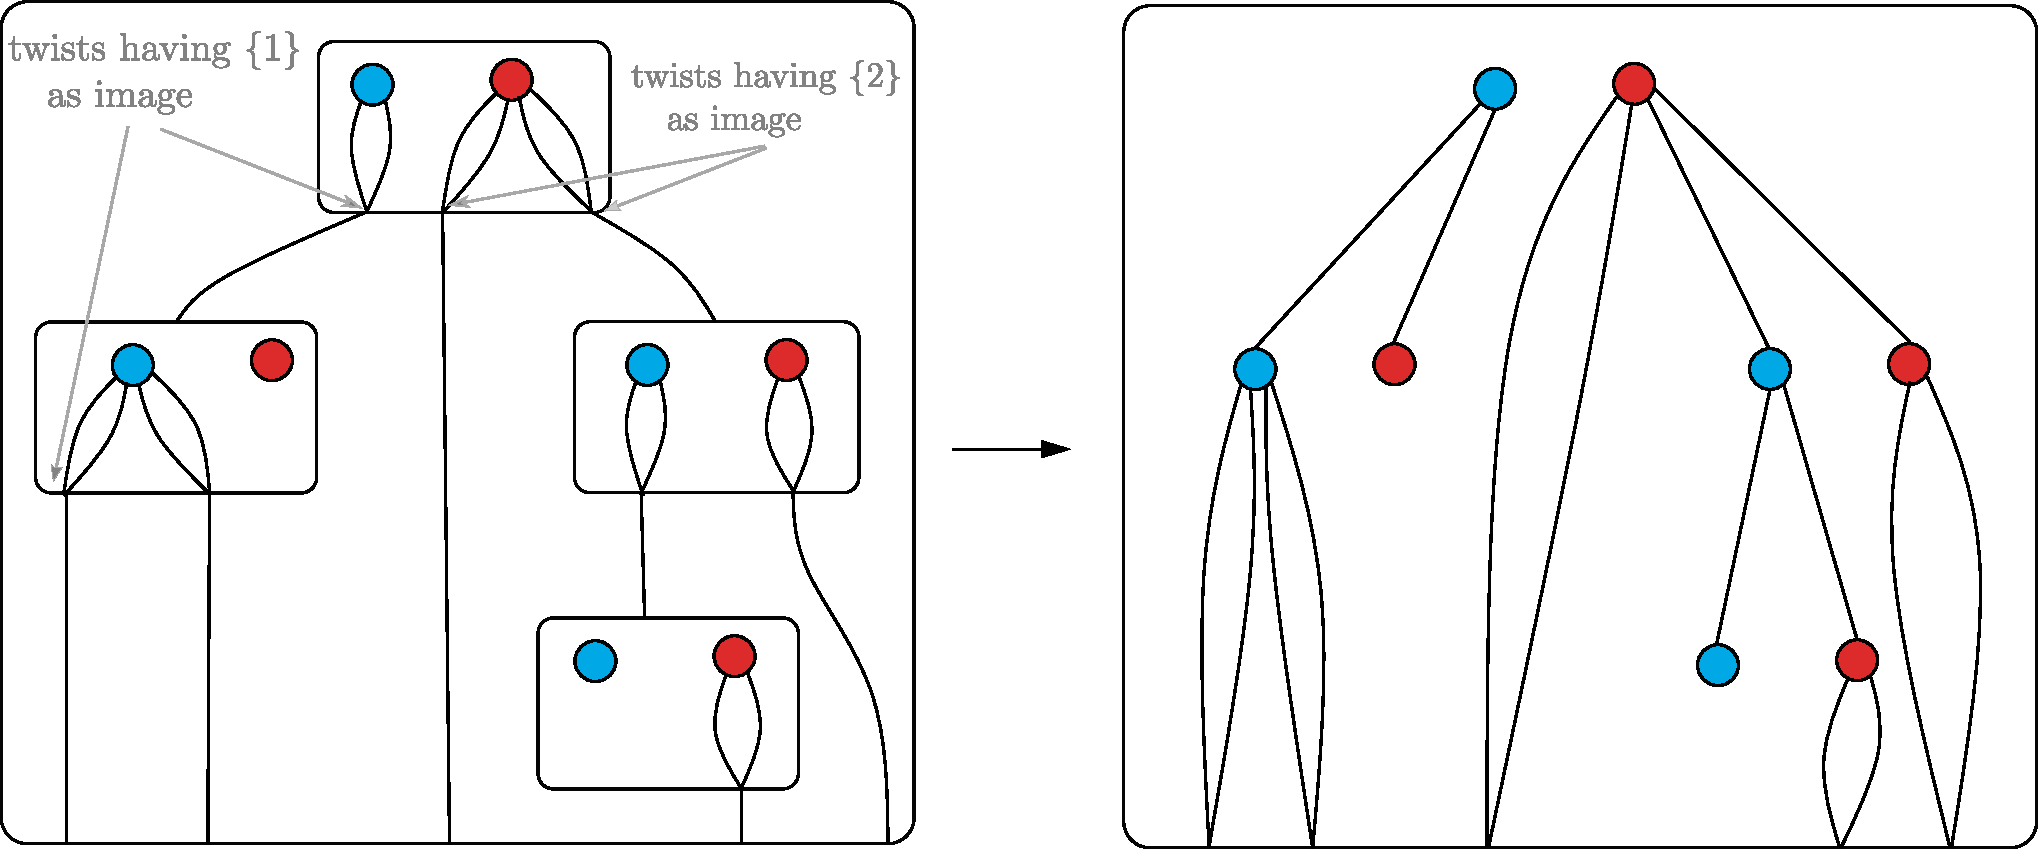
\includegraphics[scale=.3]{one-unfold.pdf}
 \end{center}
The function $f$ can be implemented by a derivable function, which we construct using following steps. We use the example above as a running example to illustrate our construction.
\begin{itemize}
 \item We start by unfolding the external twits using the corresponding basic function. We get a term in $\ranked{\reduce k \tmonad \Sigma^{[k]}}$. Our example becomes like this
   \begin{center}
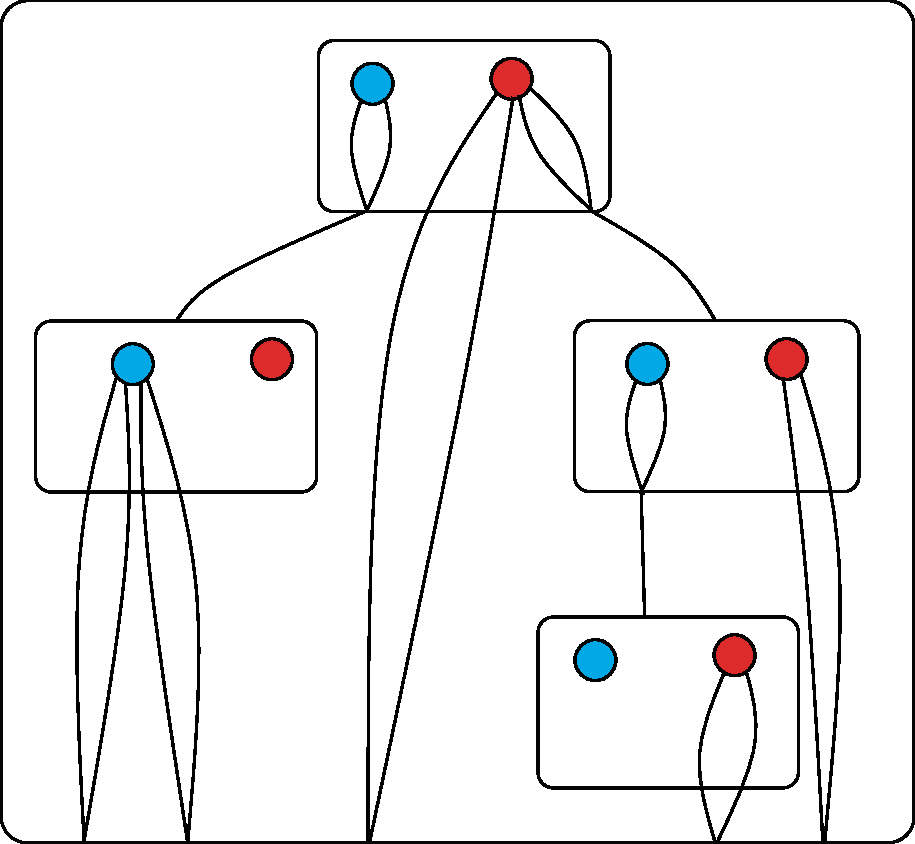
\includegraphics[scale=.3]{one-unfold1.pdf}
 \end{center}
 \item Next, we will transform each matrix power node into a tensor product as follows 
 \begin{align*}
 \ranked{ \Sigma^{[k]} \rightarrow \reduce k (\reduce k \Sigma \otimes \dots \reduce k \Sigma) \to \reduce 1 (\reduce k \Sigma)^k}
 \end{align*}
 The idea here is that, since the image of each twist is a singleton,  the ports of the matrix power are independent. We can then transform safely each node into a tensor product. After that, we transform each tensor product $\ranked{(\reduce k \Sigma)^k}$ into a shallow term $\ranked{k.\reduce k \Sigma}$ which we see itself as a term of type $\ranked{\tmonad(k+\reduce k\Sigma)}$. After the application of the unfolding function $\mathrm{unfold}_1$ followed by a flattening, and the simplification of $\ranked{\reduce k \reduce 1 \tmonad (k+\reduce k \Sigma)}$ into $\ranked{\reduce k \tmonad (k+\reduce k \Sigma)}$ we get a term in $\ranked{\reduce k \tmonad(k+\reduce k \Sigma)}$. Our running example becomes as follows after this step
   \begin{center}
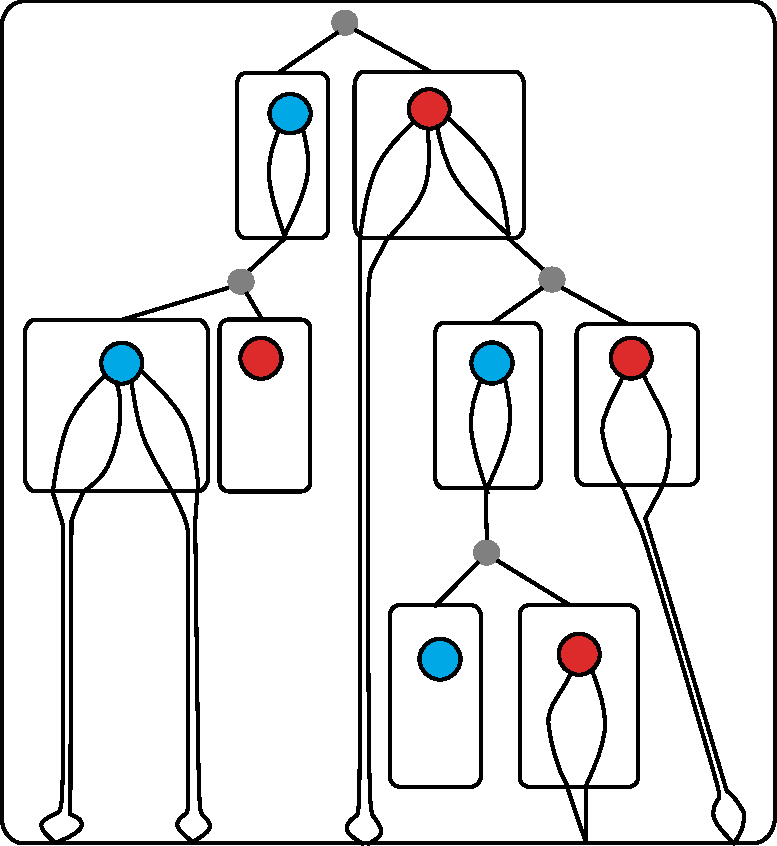
\includegraphics[scale=.3]{one-unfold2.pdf}
 \end{center}
 \item Now we apply the factorization 
 \begin{align*}
 \ranked{\tmonad (k + \reduce k \Sigma)\to \tmonad \tmonad(k + \reduce k \Sigma)}
 \end{align*}
 which regroups each element $\ranked{\reduce k \Sigma}$ with its children of type $\ranked{k}$ in the same factor, and leaves the other nodes in isolated factors. At this point our term looks like this
   \begin{center}
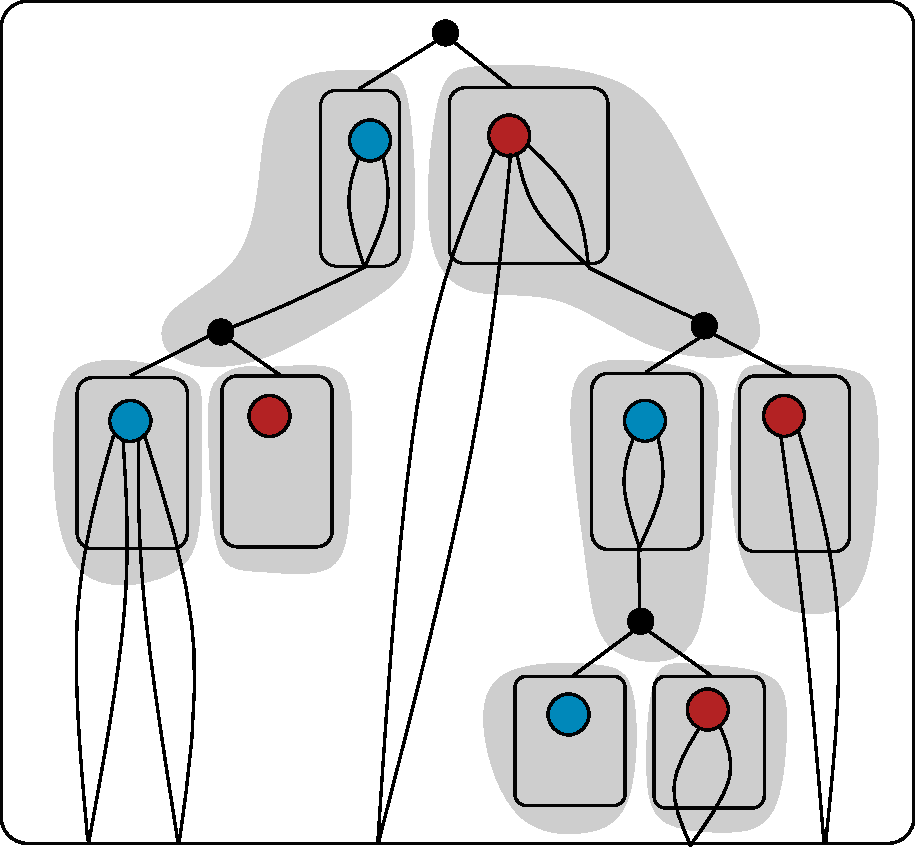
\includegraphics[scale=.3]{one-unfold3.pdf}
 \end{center}
 Note that we have two kind of factors: the first is a singleton and contains only a node labeled by $\ranked{k}$, the other kind of factors are those partial shallow terms $\ranked{(\reduce k \Sigma) * k}$. The idea now is to reflect this distinction in the type. That is to apply the function
 \begin{align*}
 \ranked{\tmonad \tmonad(k + \reduce k \Sigma) \to k. \tmonad ((\reduce k \Sigma)*k)}
 \end{align*}
 This function can be implemented easily using the decomposition function, the functions which maps every type to $\ranked{\bot}$ and mechanisms of raising errors. 
 \item Now the idea is to transform each node $\ranked{(\reduce k \Sigma)*k}$ into a $\rSigma$ one. We do so by transforming $\ranked{k}$ into $\ranked{1^k}$ (this function is basic since its domain is finite), then by applying the partial shallow unfold function of Example~\ref{ex:partial-shallow-unfold}, as illustrated by the following picture
   \begin{center}
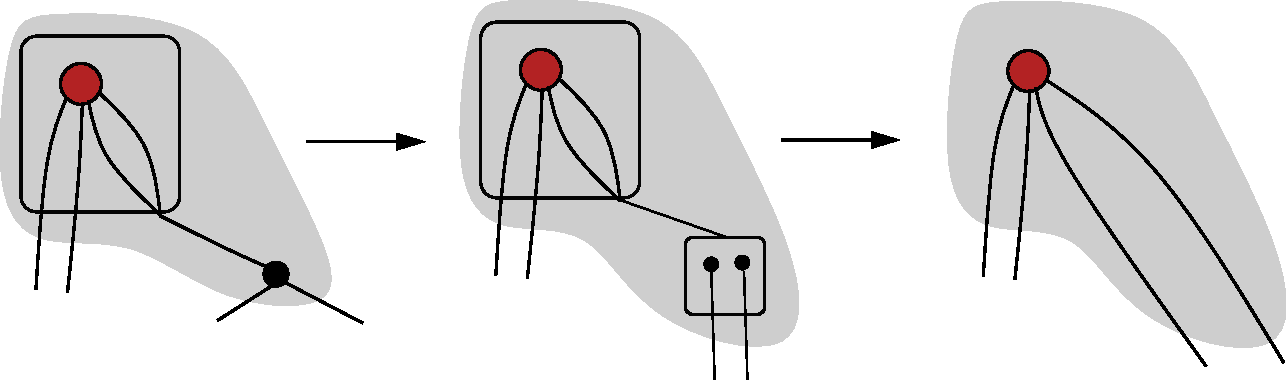
\includegraphics[scale=.3]{one-unfold4.pdf}
 \end{center}
 \end{itemize}
\end{example}
